At this point we are confronted with a problem. The best estimate of the correlator is an average over the number of thermalized
configurations, but each \textit{next} configuration is generated, site by site, from the \textit{previous}. In other words, the configurations corresponding to subsequent
sweeps are not independent: the observables $\ct_{n}$ are correlated in Markovian time $n$.
As a consequence, in the limit $N_{sweep}\to\infty$, the variance of our numerical computation is
\begin{align}
\sigma ^2\qty[\overline\ct] = \frac{\sigma ^2\qty[\ct]}{N_{sweep}}\qty{1 + 2\sum_{n=1}^{\infty}\frac{\Gamma_{\t}(n)}{\Gamma_{\t}(0)}}
\end{align}
where $\Gamma_{\t}(n) \equiv \ev{\ct_{m} \ct_{m+n}}_{m}-\overline{\ct}^2$ is the autocorrelation function at (Markovian) time $n$\footnote{It is worth noting that $\Gamma_{\t}(0) = \sigma ^2[\ct]$}.
The ratio $\nicefrac{\Gamma_{\t}(n)}{\Gamma_{\t}(0)}$ is a measure of the correlation between two observables $\ct_{m}$ that are $n$ sweeps apart\footnote{$n$ is also known as \textit{lag}.}. Indeed, if the ratio was $0$ we would recover the variance on the mean of uncorrelated measures that we would expect.

For a Markov chain,
\begin{align}
  \label{eqn:autoratio}
  \frac{\Gamma_{\t}(n)}{\Gamma_{\t}(0)} \sim \exp\qty(-\frac{n}{\tau});
\end{align}
we call $\tau$ the \textit{autocorrelation time} and note that after $\sim 4,5 \tau$ sweeps the correlation between two observables becomes
negligible.
\begin{figure}[ht]
  \centering
  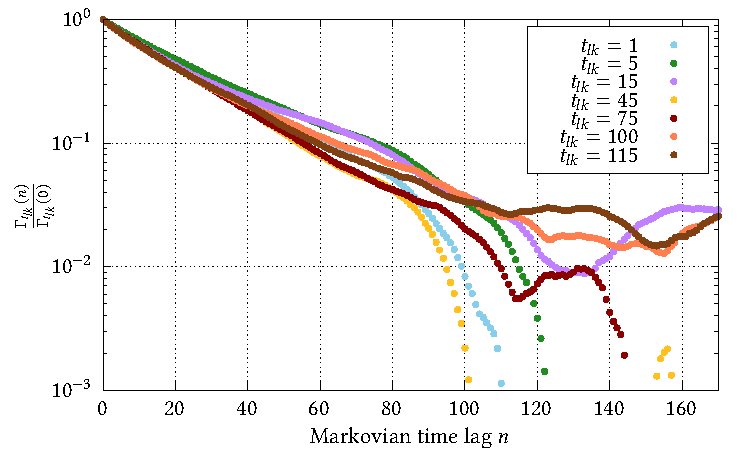
\includegraphics[width=\linewidth]{gamma.pdf}
  \caption{\label{fig:gammat} Autocorrelation  as a function of Markovian lag for observables at different fixed physical times. Its value decreases exponentially with $n$ -- $y$ axis is in $\log$ scale -- until it starts oscillating. Observables corresponding to larger physical times (equivalent to the distance of the sites on the lattice) need more sweeps to
  decorrelate.}
\end{figure}
Therefore, it is possible to decorrelate the measures through a binning procedure, in order to minimize the impact of consequent Feynman paths.
The value of $\tau$ can be determined from an exponential fit of ratio \ref{eqn:autoratio} and used to group
$D_{bin}\sim 10,100\tau$ observables together in a single bin, of which we take the average value.
As a consequence, we will now work with $N_{bin}=\nicefrac{N_{sweep}}{D_{bin}}$ decorrelated observables
\begin{align}
  \label{eqn:binned}
  \ct_{n}= \frac{1}{D_{bin}}\sum_{j=1}^{D_{bin}}\ct_{j}; \, n = 1, \dots, N_{bin}
\end{align}
on which we can apply the \textit{usual} statistical analysis over $N_{bin}$ Feynman paths, thus obtaining the best estimation of the correlator \ref{eqn:integral} as
\begin{align}
  \label{eqn:bestestim}
  \ct = \frac{1}{N_{bin}}\sum_{n=1}^{N_{bin}}\ct_{n},
\end{align}
with variance\footnote{The binning procedure on $x^{2}$ happened \textit{after} the coordinates were squared.}
\begin{align}
  \label{eqn:bestvariance}
  \sigma^{2}\qty[\ct] = \frac{1}{N_{bin}}\qty[\ev{x_{l,binned}^{2}x_{k,binned}^{2}}-\ct^{2}].
\end{align}
\begin{figure}[h]
  \centering
  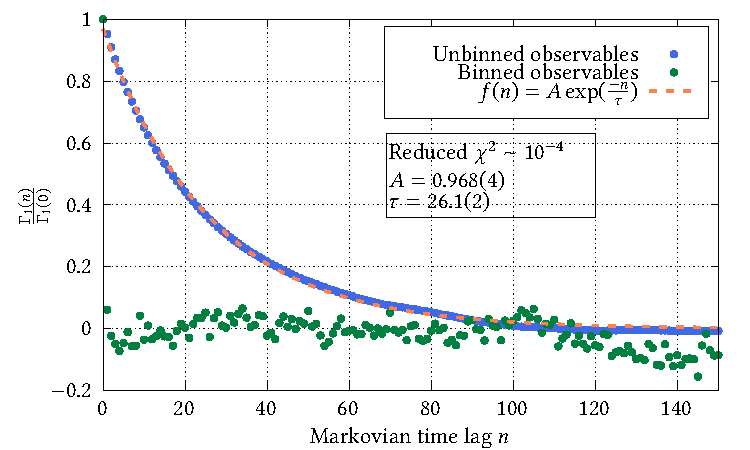
\includegraphics[width=\linewidth]{binvsnot}
  \caption{\label{fig:binvsnot}Autocorrelation for binned and unbinned correlators; the exponential fit has been done with Gnuplot. The value of $\tau=26$ was then used to determine the bin width
    $D_{bin}=500$. The binned observables, shown here in green,
  are decorrelated from the start.}
\end{figure}
\\
In figure \ref{fig:binvsnot} we show the autocorrelation for both the unbinned and the binned correlator at $\t = 1$. It takes
$\tau \sim 26$ sweeps for the unbinned observables' autocorrelation to decrease to $\nicefrac{1}{e}$, therefore we set $D_{bin}=500$. As expected,
the binned observables among different sweeps are not correlated from the start.

